\documentclass[tikz,border=4pt]{standalone}
\usepackage{amsmath,amssymb}
\usetikzlibrary{arrows.meta}
\begin{document}
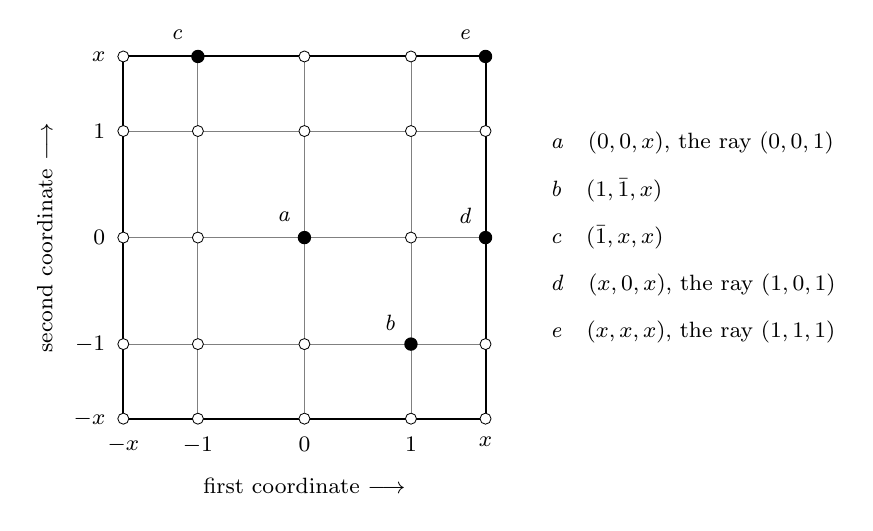
\begin{tikzpicture}[line cap=round,line join=round]
\draw[line width=0.7pt] (-2.3000,-2.3000) -- (-2.3000,2.3000);
\draw[line width=0.7pt] (-2.3000,-2.3000) -- (2.3000,-2.3000);
\draw[line width=0.3pt,gray] (-1.3529,-2.3000) -- (-1.3529,2.3000);
\draw[line width=0.3pt,gray] (-2.3000,-1.3529) -- (2.3000,-1.3529);
\draw[line width=0.3pt,gray] (0.0000,-2.3000) -- (0.0000,2.3000);
\draw[line width=0.3pt,gray] (-2.3000,0.0000) -- (2.3000,0.0000);
\draw[line width=0.3pt,gray] (1.3529,-2.3000) -- (1.3529,2.3000);
\draw[line width=0.3pt,gray] (-2.3000,1.3529) -- (2.3000,1.3529);
\draw[line width=0.7pt] (2.3000,-2.3000) -- (2.3000,2.3000);
\draw[line width=0.7pt] (-2.3000,2.3000) -- (2.3000,2.3000);
\draw[fill=white,line width=0.3pt] (-2.3000,-2.3000) circle (0.070);
\draw[fill=white,line width=0.3pt] (-2.3000,-1.3529) circle (0.070);
\draw[fill=white,line width=0.3pt] (-2.3000,0.0000) circle (0.070);
\draw[fill=white,line width=0.3pt] (-2.3000,1.3529) circle (0.070);
\draw[fill=white,line width=0.3pt] (-2.3000,2.3000) circle (0.070);
\draw[fill=white,line width=0.3pt] (-1.3529,-2.3000) circle (0.070);
\draw[fill=white,line width=0.3pt] (-1.3529,-1.3529) circle (0.070);
\draw[fill=white,line width=0.3pt] (-1.3529,0.0000) circle (0.070);
\draw[fill=white,line width=0.3pt] (-1.3529,1.3529) circle (0.070);
\draw[fill=white,line width=0.3pt] (-1.3529,2.3000) circle (0.070);
\draw[fill=white,line width=0.3pt] (0.0000,-2.3000) circle (0.070);
\draw[fill=white,line width=0.3pt] (0.0000,-1.3529) circle (0.070);
\draw[fill=white,line width=0.3pt] (0.0000,0.0000) circle (0.070);
\draw[fill=white,line width=0.3pt] (0.0000,1.3529) circle (0.070);
\draw[fill=white,line width=0.3pt] (0.0000,2.3000) circle (0.070);
\draw[fill=white,line width=0.3pt] (1.3529,-2.3000) circle (0.070);
\draw[fill=white,line width=0.3pt] (1.3529,-1.3529) circle (0.070);
\draw[fill=white,line width=0.3pt] (1.3529,0.0000) circle (0.070);
\draw[fill=white,line width=0.3pt] (1.3529,1.3529) circle (0.070);
\draw[fill=white,line width=0.3pt] (1.3529,2.3000) circle (0.070);
\draw[fill=white,line width=0.3pt] (2.3000,-2.3000) circle (0.070);
\draw[fill=white,line width=0.3pt] (2.3000,-1.3529) circle (0.070);
\draw[fill=white,line width=0.3pt] (2.3000,0.0000) circle (0.070);
\draw[fill=white,line width=0.3pt] (2.3000,1.3529) circle (0.070);
\draw[fill=white,line width=0.3pt] (2.3000,2.3000) circle (0.070);
\node[below=3pt,font=\footnotesize] at (-2.3000,-2.3000) {$-x$};
\node[left=3pt,font=\footnotesize] at (-2.3000,-2.3000) {$-x$};
\node[below=3pt,font=\footnotesize] at (-1.3529,-2.3000) {$-1$};
\node[left=3pt,font=\footnotesize] at (-2.3000,-1.3529) {$-1$};
\node[below=3pt,font=\footnotesize] at (0.0000,-2.3000) {$0$};
\node[left=3pt,font=\footnotesize] at (-2.3000,0.0000) {$0$};
\node[below=3pt,font=\footnotesize] at (1.3529,-2.3000) {$1$};
\node[left=3pt,font=\footnotesize] at (-2.3000,1.3529) {$1$};
\node[below=3pt,font=\footnotesize] at (2.3000,-2.3000) {$x$};
\node[left=3pt,font=\footnotesize] at (-2.3000,2.3000) {$x$};
\fill (0.0000,0.0000) circle (0.085);
\node[font=\footnotesize\itshape,fill=white,inner sep=1pt] at (-0.2700,0.2700) {a};
\node[right,font=\footnotesize] at (3.0000,1.2000) {\textit{a}\quad $(0,0,x)$, the ray $(0,0,1)$};
\fill (1.3529,-1.3529) circle (0.085);
\node[font=\footnotesize\itshape,fill=white,inner sep=1pt] at (1.0829,-1.0829) {b};
\node[right,font=\footnotesize] at (3.0000,0.6000) {\textit{b}\quad $(1,\bar 1,x)$};
\fill (-1.3529,2.3000) circle (0.085);
\node[font=\footnotesize\itshape,fill=white,inner sep=1pt] at (-1.6229,2.5700) {c};
\node[right,font=\footnotesize] at (3.0000,0.0000) {\textit{c}\quad $(\bar 1,x,x)$};
\fill (2.3000,0.0000) circle (0.085);
\node[font=\footnotesize\itshape,fill=white,inner sep=1pt] at (2.0300,0.2700) {d};
\node[right,font=\footnotesize] at (3.0000,-0.6000) {\textit{d}\quad $(x,0,x)$, the ray $(1,0,1)$};
\fill (2.3000,2.3000) circle (0.085);
\node[font=\footnotesize\itshape,fill=white,inner sep=1pt] at (2.0300,2.5700) {e};
\node[right,font=\footnotesize] at (3.0000,-1.2000) {\textit{e}\quad $(x,x,x)$, the ray $(1,1,1)$};
\node[font=\footnotesize] at (0,-3.1500) {first coordinate $\longrightarrow$};
\node[font=\footnotesize,rotate=90] at (-3.3000,0) {second coordinate $\longrightarrow$};
\end{tikzpicture}
\end{document}
